%%%%%%%%%%%%%%%%%%%%%%%%%%%%%%%%%%%%%%%%% 
% Dreuw & Deselaer's Poster
% LaTeX Template
% Version 1.0 (11/04/13)
% 
% Created by:
% Philippe Dreuw and Thomas Deselaers
% http://www-i6.informatik.rwth-aachen.de/~dreuw/latexbeamerposter.php
% 
% This template has been downloaded from:
% http://www.LaTeXTemplates.com
% 
% License:
% CC BY-NC-SA 3.0 (http://creativecommons.org/licenses/by-nc-sa/3.0/)
% 
%%%%%%%%%%%%%%%%%%%%%%%%%%%%%%%%%%%%%%%%% 

% ----------------------------------------------------------------------------------------
%	PACKAGES AND OTHER DOCUMENT CONFIGURATIONS
% ----------------------------------------------------------------------------------------

\documentclass[final,hyperref={pdfpagelabels=false}]{beamer}

\usepackage[orientation=portrait,size=a0,scale=1.18]{beamerposter} % Use the beamerposter package for laying out the poster with a portrait orientation and an a0 paper size

\usetheme{I6pd2} % Use the I6pd2 theme supplied with this template

\usepackage[english]{babel} % English language/hyphenation

\usepackage{amsmath,amsthm,amssymb,latexsym} % For including math equations, theorems, symbols, etc

% \usepackage{times}\usefonttheme{professionalfonts}  % Uncomment to use Times as the main font
% \usefonttheme[onlymath]{serif} % Uncomment to use a Serif font within math environments

\boldmath % Use bold for everything within the math environment

\usepackage{booktabs} % Top and bottom rules for tables

\graphicspath{{figures/}} % Location of the graphics files

\usecaptiontemplate{\small\structure{\insertcaptionname~\insertcaptionnumber: }\insertcaption} % A fix for figure numbering


%SEttings added by me :)
\bibliographystyle{plain}
\usepackage{multicol}
%\usepackage[document]{ragged2e}
%\usepackage{ragged2e}

% --------------------------------
% CUSTOM COMMANDS ETC.
% ---------------------------------
\renewcommand{\Re}{\operatorname{Re}}
\renewcommand{\Im}{\operatorname{Im}}
\usepackage{braket}
\newcommand{\mean}[1]{\langle #1 \rangle}


% ----------------------------------------------------------------------------------------
%	TITLE SECTION 
% ----------------------------------------------------------------------------------------

\title{\huge An Alternative to Contextuality} % Poster title

\author{Atul Singh Arora \\ \small supervisor: Prof. Arvind} % Author(s)

% \institute{{\small Quantum Computation \& Quantum Information (QCQI) Group,} Indian Institute of Science Education \& Research (IISER), Mohali} % Institution(s)
\institute{Indian Institute of Science Education \& Research (IISER), Mohali} % Institution(s)

% ----------------------------------------------------------------------------------------
%	FOOTER TEXT
% ----------------------------------------------------------------------------------------

\newcommand{\leftfoot}{}  %http://www.LaTeXTemplates.com} % Left footer text

\newcommand{\rightfoot}{} %john@smith.com} % Right footer text

% ----------------------------------------------------------------------------------------

\begin{document}

\addtobeamertemplate{block
  end}{}{\vspace*{1ex}} % White space under blocks

%\justify
\begin{frame}[t] % The whole poster is enclosed in one beamer frame

  \begin{columns}[c] % The whole poster consists of two major columns, each of which can be subdivided further with another \begin{columns} block - the [t] argument aligns each column's content to the top

    \begin{column}{.015\textwidth}\end{column} % Empty spacer column
    \begin{column}{.31\textwidth} % The first column


      \setbeamercolor{block title}{fg=taorange,bg=ta2gray}
      %\setbeamercolor{block title}{fg=black,bg=orange!70} % Change the block title color


      % ----------------------------------------------------------------------------------------
      % BACKGROUND
      % ----------------------------------------------------------------------------------------
      \begin{block}{I. Background}
        \begin{columns}
          \begin{column}{0.7\textwidth}
            \begin{itemize}
            \item Einstein: `locality' $\implies$ Quantum Mechanics (QM) is incomplete \cite{EPR}. 

            \item Bell: `locality'  $\implies \mean {\hat B} \le 2$; For some $\ket{\psi}$, QM $\implies \mean{\hat B} = 2\sqrt 2$ \cite{Bell}. Verified experimentally (without loop holes in 2015)

            \item Comment: At roughly the same time, various physicists had produced proofs of the claim that one can't complete QM satisfactorily, that a sensible complete `hidden variable' (HV) description of nature was impossible. 

            \item Bohmian Mechanics (BM): a HV description, that (i) `completes' QM in a simple, clear, precise but non-local manner, and (ii) is deterministic \cite{bohm1}.

            \item Defn: \emph{Deterministic} $\equiv$ If in principle, the outcome of measuring each observable is predictable, given the HVs. %Probabilities enter the description because of our ignorance and is not intrinsic to nature.

            \item Comment: Bell's inequality requires entanglement in some form, to prove Einstein's notion of locality incorrect. Recently, another peculiar feature of QM has been identified, namely contextuality. 

            \item Impl Defn: \emph{Context} $\equiv$ If $[\hat A,\hat B]=0$ and $[A,C]=0$ but $[B,C]\neq 0$, then possible contexts are {A}, {A and B} or {A and C} \cite{peresBook}.

            \item Defn: \emph{Non-contextual} $\equiv$ Value an operator takes, depends only on the state (including `hidden variables') and the choice of the operator $A$ (not it's context) \cite{peresBook}.

            \item Defn: \emph{Contextual} $\equiv$ Value an operator takes, depends on it's context \cite{peresBook}.

            \item Comment: This notion arises, atleast in certain explicit constructions, where one is unable to assign values to operators, consistent with predictions of QM.

            \item Aim: Understand how a deterministic theory can be consistent with the notion of contextuality.

            \end{itemize}
          \end{column}

          \begin{column}{0.3\textwidth}
            \begin{figure}
              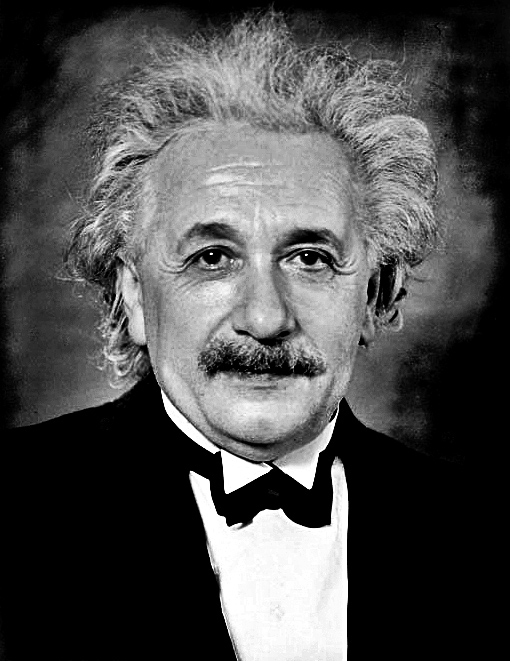
\includegraphics[width=0.8\linewidth]{einstein}
              \caption{A. Einstein}
            \end{figure}
            \begin{figure}
              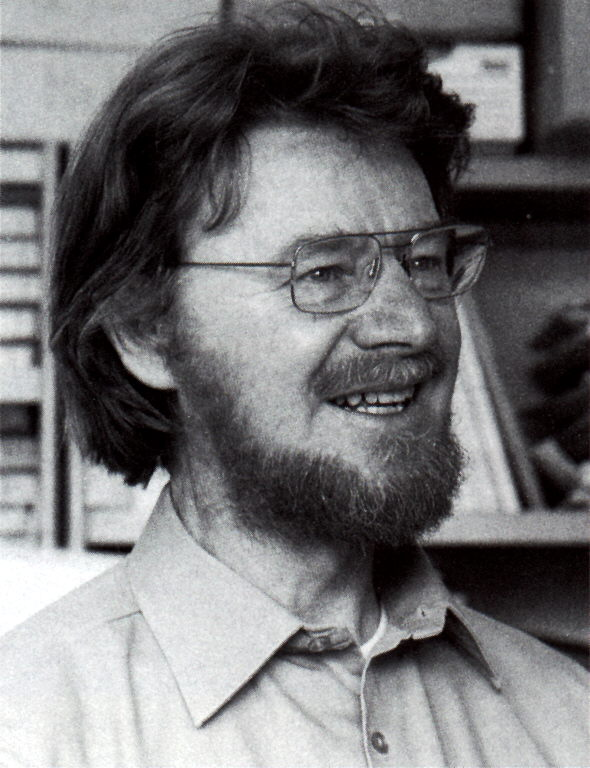
\includegraphics[width=0.8\linewidth]{bell}
              \caption{J. Bell}
            \end{figure}
            \begin{figure}
              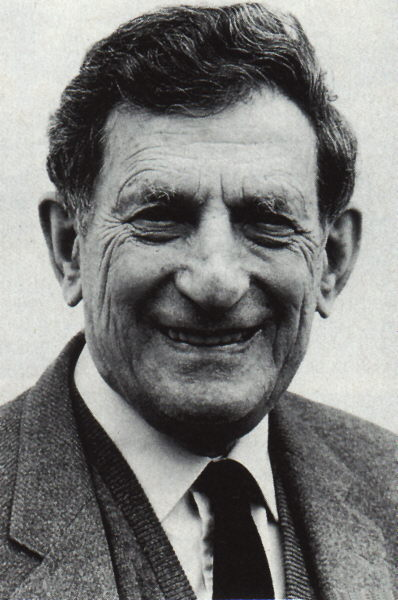
\includegraphics[width=0.8\linewidth]{bohm}
              \caption{D. Bohm}
            \end{figure}
            \begin{figure}
              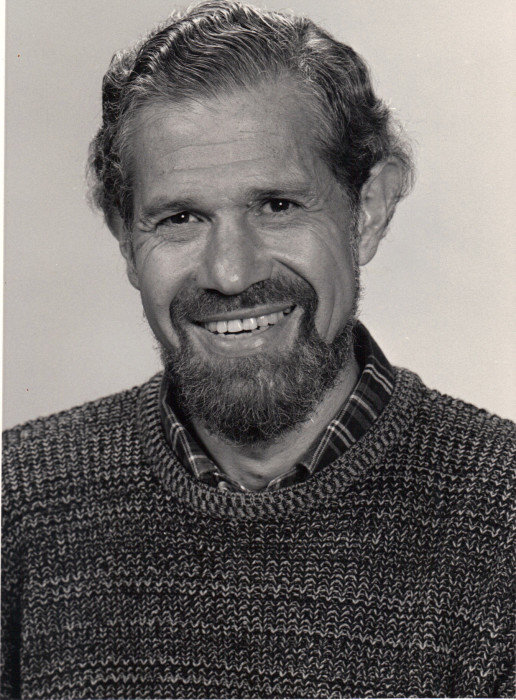
\includegraphics[width=0.8\linewidth]{kochen}
              \caption{S. B. Kochen}
            \end{figure}

          \end{column}
        \end{columns}
      \end{block}

      % ----------------------------------------------------------------------------------------
      % OVERVIEW
      % ----------------------------------------------------------------------------------------
      
      \begin{block}{II. Overview}

            \begin{figure}
              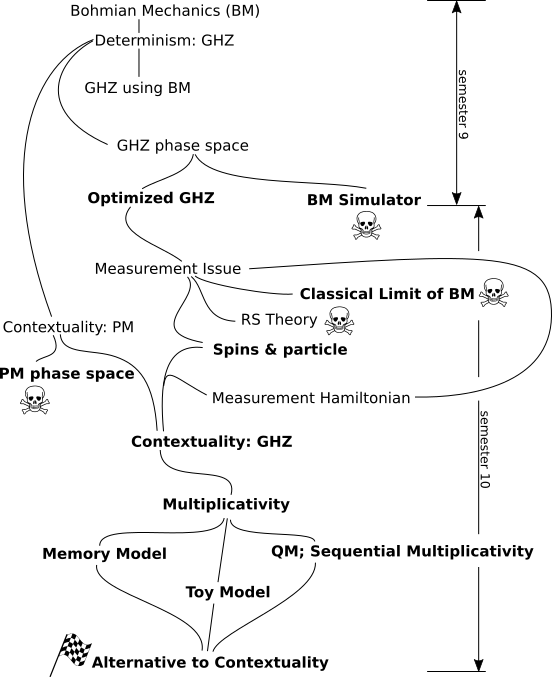
\includegraphics[width=0.99\linewidth]{flow.png}
              \caption{Exploration flow: Boldface titles represent new results}
            \end{figure}

      \end{block}


      % \setbeamercolor{block title}{fg=taorange,bg=ta2gray}
      \setbeamercolor{block title}{fg=black,bg=orange!70} % Change the block title color

      % ----------------------------------------------------------------------------------------
      % ACKNOWLEDGEMENTS
      % ----------------------------------------------------------------------------------------

      \begin{block}{Early Acknowledgments}
        I thank Prof. Arvind, for facilitating the completion of this project, by providing necessary resources and guidance. Discussions with Mr. Rajendra Bhati and Mr. Kishor Bharti have been particularly efficacious. Jaskaran Singh has also provided valuable inputs. The KVPY programme, DST, and IISER Mohali are duly acknowledged for providing financial, infrastructural and research education support.
      \end{block}

      \setbeamercolor{block title}{fg=taorange,bg=ta2gray}
      % \setbeamercolor{block title}{fg=black,bg=orange!70} % Change the block title color


    \end{column}

    %\begin{column}{.005\textwidth}\end{column} % Empty spacer column    
    \begin{column}{.69\textwidth}
      \begin{columns}[c]

        \begin{column}{.012\textwidth}\end{column} % Empty spacer column
        \begin{column}{.48\textwidth} % The first column


          % ----------------------------------------------------------------------------------------
          % Multiplicativity
          % ----------------------------------------------------------------------------------------

          \begin{block}{III. Multiplicativity}
            \begin{itemize}

            \item Defn: \emph{Compatible operators} $\equiv$ Two observables $\hat A$ and $\hat B$ are mutually compatible if, given that the system is prepared in a state s.t. measurement $\hat A$ yields repeatable results, measurement of $\hat B$ doesn't change the result of measuring $\hat A$. For projective measurements, its equivalent to $[\hat A, \hat B]=0$. %  the result of measuring $A$ doesn't depend on whether $B$ is measured (before, after, simultaneously or not measured at all). TODO: Update this definition.
              
            \item Defn: \emph{Multiplicativity} $\equiv$ For compatible operators $\hat{B_i}$, a model is multiplicative iff 
              \begin{align} f(m_1(\hat{B}_1),m_1(\hat{B}_2),&\dots,m_1(\hat{B}_n)) = \\
                                                            &m_1(f(\hat{B}_1,\hat{B}_2,\dots,\hat{B}_n),
              \end{align}
              where $m_j(\hat *)$ represents the assigned value of the operator, and $j$ encodes the sequence of measurement. Note that this is an ontological statement and can't be experimentally tested.

            \item Defn: \emph{Sequential Multiplicativity} $\equiv$ For compatible operators $\hat{B_i}$, a model is sequentially multiplicative iff 
              \begin{align} f(m_{k_1}(\hat{B}_1),m_{k_2}(\hat{B}_2),&\dots,m_{k_n}(\hat{B}_n)) = \\
                                                                    &m_1(f(\hat{B}_1,\hat{B}_2,\dots,\hat{B}_n),
              \end{align}
              where $\mathbf k \equiv (k_1,k_2,\dots,k_n) \in ((1,2,\dots,n)$ + all possible permutations $)$, $m_j(\hat *)$ represents the assigned value of the operator, and $j$ encodes the sequence of measurement.

            \item Example: $\hat B_1 = \hat {\sigma} _x \otimes \hat {\sigma}_y$, $\hat B_2 = \hat {\sigma} _y \otimes \hat {\sigma}_x$ so that $\hat C = \hat B_1 \hat B_2 = \hat \sigma _z \otimes \hat \sigma _z$. $\ket {\psi}=\ket{00}$, so that $m_1(\hat C)=1$, while $m_1(\hat B_i)=\pm 1$. If say $m_1(\hat B_1)=-1$, then ${\psi} \to \text{(figure this)}$ so that entails $m_2(\hat B_2)=-1$ as well, consistent with $m_1(\hat C)=m_1(\hat B_1)m_2(\hat B_2)$.

            \item Claim: Quantum Mechanics is sequentially multiplicative.

            \end{itemize}

          \end{block}

        \end{column}

        %\begin{column}{.005\textwidth}\end{column} % Empty spacer column
        \begin{column}{.46\textwidth}

          % ----------------------------------------------------------------------------------------
          % Contextuality - PM TEST
          % ----------------------------------------------------------------------------------------
          \begin{block}{IV. Contextuality - PM Test}

            %Defn: \emph{Non-contextually Deterministic} $\equiv$ If we restrict ourselves to hidden variable models that assert that $A$ and $B$ have predefined values, irrespective of which compatible observable is measured, then such a theory would be termed ``non-contextual'' and deterministic. 

            Kochen-Specker proved that non-contextual theories, are inconsistent with QM \cite{Koc}. Mermin and Peres showed this for a four-level system \cite{PeresContext}.
            \begin{itemize}
            \item Simplified Proof: Consider the following operators. 
              \[
              A_{ij} \doteq \left[
                \begin{array}{ccc}
                  \sigma_z\otimes \mathbb I &  \mathbb I \otimes \sigma_z & \sigma_z\otimes \sigma_ z \\
                  \mathbb I \otimes \sigma_x &  \sigma_x \otimes \mathbb I & \sigma_x\otimes \sigma_x \\
                  \sigma_z \otimes \sigma_x &  \sigma_x \otimes \sigma_z & \sigma_y\otimes \sigma_y
                \end{array} \right]
              \]


              Note that operators along a given row (column) commute. 
              
              \begin{align}
                R_i\equiv \prod_j A_{ij} & = \mathbb{I} \\
                C_j\equiv \prod_i A_{ij} & = 
                                           \begin{cases} 
                                             +\mathbb{I} &  (j\neq 3)\\
                                             -\mathbb{I} &  (j=3)
                                           \end{cases} 
              \end{align}
              It entails that $\prod_{k=1,2,3}R_kC_k= -\mathbb{I}$, whereas non-contextual models would yield +1.

              NB: We also assumed multiplicativity. 

              To facilitate experimental validation, it has been shown that non-contextual models satisfy Eq. \ref{eq:pm}, while QM yields $\mean{\chi_{PM}}=6$.
              \begin{equation}
                \mean{\chi_{PM}} = \mean{R_1} + \mean{R_2} + \mean{R_3} + \mean{C_1} + \mean{C_2} - \mean{C_3} \le 4
                \label{eq:pm}
              \end{equation}

            \item Conclusion: Deterministic theories, that satisfy both (a) non-contextuality and (b) multiplicativity, are inconsistent with QM.
            \end{itemize}

          \end{block}

        \end{column}

        \begin{column}{.015\textwidth}\end{column} % Empty spacer column
      \end{columns}






      \begin{columns}[c]

        \begin{column}{.005\textwidth}\end{column} % Empty spacer column
        \begin{column}{.94\textwidth} % The first column
          % ----------------------------------------------------------------------------------------
          % Toy Model | example
          % ----------------------------------------------------------------------------------------

          \begin{block}{The Toy Model | Example}
            {\small
              \begin{equation}
                \begin{array}{c|ccc}
                  \text{Iteration} & i=1 & i=2 & i=3\\
                  \left|\psi_{\text{init}}\right\rangle  & \left|00\right\rangle  & \left|00\right\rangle  & \frac{\left|00\right\rangle +\left|11\right\rangle }{\sqrt{2}}\\
                  \text{HV/Toss} & c=-1 & c=-1 & c=+1\\
                  \\
                  \text{Predictions} & m_{1}(\hat{A}_{ij})\doteq\left[\begin{array}{ccc}
                                                                        -1 & -1 & -1\\
                                                                        -1 & -1 & -1\\
                                                                        -1 & -1 & +1
                                                                      \end{array}\right] & m_{2}(\hat{A}_{ij})\doteq\left[\begin{array}{ccc}
                                                                                                                            -1 & -1 & -1\\
                                                                                                                            -1 & -1 & -1\\
                                                                                                                            -1 & -1 & +1
                                                                                                                          \end{array}\right] & m_{3}(\hat{A}_{ij})\doteq\left[\begin{array}{ccc}
                                                                                                                                                                                +1 & +1 & +1\\
                                                                                                                                                                                +1 & +1 & -1\\
                                                                                                                                                                                +1 & +1 & +1
                                                                                                                                                                              \end{array}\right]\\
                  \text{(Assignments)}\\
                                   & m_{1}(\hat{R}_{i}),m_{1}(\hat{C}_{j})=+1\,(j\neq3) & m_{2}(\hat{R}_{i}),m_{2}(\hat{C}_{j})=+1\,(j\neq3) & m_{3}(\hat{R}_{i}),m_{3}(\hat{C}_{j})=+1\,(j\neq3)\\
                                   & m_{1}(\hat{C}_{3})=-1 & m_{2}(\hat{C}_{3})=-1 & m_{3}(\hat{C}_{3})=-1\\
                  \text{Operator}\\
                  \text{Measured} & \hat{A}_{13}=\hat{\sigma}_{z}\otimes\hat{\sigma}_{z};m_{1}(\hat{A}_{13})=+1 & \quad\quad\hat{A}_{23}=\hat{\sigma}_{y}\otimes\hat{\sigma}_{y};m_{2}(\hat{A}_{23})=-1\quad\quad & \hat{A}_{33}=\hat{\sigma}_{x}\otimes\hat{\sigma}_{x};m_{3}(\hat{A}_{33})=+1\\
                  \\
                  \left|\psi_{\text{final}}\right\rangle  & \left|00\right\rangle  & \frac{\left|00\right\rangle +\left|11\right\rangle }{\sqrt{2}} & \frac{\left|00\right\rangle +\left|11\right\rangle }{\sqrt{2}}
                \end{array}
              \end{equation}}
          \end{block}


        \end{column}

        \begin{column}{.015\textwidth}\end{column} % Empty spacer column
      \end{columns}














      \begin{columns}[b]

        \begin{column}{.012\textwidth}\end{column} % Empty spacer column
        \begin{column}{.48\textwidth} % The first column

          % ----------------------------------------------------------------------------------------
          % Memory Model
          % ----------------------------------------------------------------------------------------

          \begin{block}{V. Contextuality - Memory Model}
              An example of a contextual and non-multiplicative model; Sequential multiplicativity has been assumed.

            \begin{itemize}
              \item Initial: The assignment is as given in the first Mat in Eq. \ref{eq:allPlus}. 

              \item Remark: The system is assumed to be capable of remembering the last three observables that were measured. 

              \item Algorithm: Upon measurement of an observable, (i) yield the value as saved in the matrix, (ii) append the observable in the 3 element memory and (iii) update the matrix, once the context (set of commuting observables) is known, to satisfy the PM requirements.
                \begin{align}  \label{eq:allPlus} 
                  m_1(\hat A_{ij})=m_2 (\hat A_{ij})\doteq
                  \left[
                  \begin{array}{ccc}
                    1 & 1 & 1 \\
                    1 & 1 & 1 \\
                    1 & 1 & 1
                  \end{array} \right],
                            &
                              m_3 (\hat A_{ij}) \doteq
                              \left[
                              \begin{array}{ccc}
                                1 & 1 & -1 \\
                                1 & 1 & 1 \\
                                1 & 1 & 1
                              \end{array}\right] %\label{eq:oneMinus}
                \end{align}

              \item For example:
                \[
                \begin{array}{c|ccc}
                  \text{Operator} & \text{Updated Array} & \text{Assignment} & \text{Value}\\
                  \hat {A}_{33} & \{*,*,\hat{A}_{33}\} & m_1(\hat A_{ij}) & 1\\
                  \hat {A}_{23} & \{*,\hat{A}_{33},\hat{A}_{23}\} & m_2(\hat A_{ij}) & 1\\
                  \hat {A}_{13} & \{\hat{A}_{33},\hat{A}_{23},\hat {A}_{13}\} & m_3(\hat A_{ij}) & -1
                \end{array}
                \]

                Result: $m_1(C_3)=-1$ as required.
              \end{itemize}
          \end{block}

          % ------------------------------------------------
          % The Toy Model
          % ------------------------------------------------
          \begin{block}{VI. The Toy Model}
            An example of a non-contextual non-multiplicative model; Sequential multiplicativity is demonstrated.
            \begin{itemize}
              \item Initial: $\ket {\psi}$.
              \item `hidden variable': Choose $c=+1$ for heads, $c=-1$ for tails, after a coin toss.
              \item Predictions/Assignments: For an operator $\hat{p}'\in\{\hat{A}_{ij},\hat{R}_{i},$ + their products such as $\hat{C}_{j}\,(\forall\,i,j)\}$  check if $\exists$ a $\lambda$, s.t. $\hat{p}'\left|\psi\right\rangle =\lambda\left|\psi\right\rangle$. If $\exists$ a $\lambda$, then assign $\lambda$ as the value. Else, assign c.
              \item Update: Say $\hat{p}$ was observed. If $\hat{p}$ is s.t. $\hat{p}\left|\psi\right\rangle =\lambda\left|\psi\right\rangle$, then leave the state unchanged. Else, find $\left|p_{\pm}\right\rangle$   (eigenkets of $\hat{p}$), s.t. $\hat{p}\left|p_{\pm}\right\rangle =\pm\left|p_{\pm}\right\rangle$ and update the state $\left|\psi\right\rangle \to\left|p_{c}\right\rangle$. 
            \end{itemize}
            NB: This would statistically agree with QM, for a few $\ket{\psi}$s.
          \end{block}

          % ----------------------------------------------------------------------------------------

        \end{column}

        %\begin{column}{.005\textwidth}\end{column} % Empty spacer column
        \begin{column}{.47\textwidth}


          % ----------------------------------------------------------------------------------------
          % CONCLUSION
          % ----------------------------------------------------------------------------------------

          \begin{block}{VII. Results and Conclusion}
            \begin{itemize}
            \item Contextuality is not necessary.
              {\tiny
              \begin{itemize}
              \item The properties `multiplicativity' and `sequential multiplicativity' were identified, defined and proven where they hold.
              \item Demonstrated that `non-multiplicativity' is an alternative to `contextuality', by constructing a `non-contextual' theory, consistent with QM predictions.
              \item Proposed a Minimalistic HV theory; simplifies predictions.
              \end{itemize}}
            \item Tests of Determinism and Contextuality
              {\tiny
              \begin{itemize}
                \item Optimized phase-space GHZ
                \item GHZ extension to a test of contextuality
                \item PM extension to phase space (independently re-discovered)
              \end{itemize}}
            \item Measurements in Bohmain Mechanics
              {\tiny
              \begin{itemize}
                \item Generalized the Hamiltonian based measurement scheme to continuous variables
                \item Analytic/graphical solution to measuring entangled spins using SG
                \item Analytic/graphical proof of consistency of position measurements
                \item Alternative proof of spins can't be associated with particles, only with wavefunctions
              \end{itemize}}
            \end{itemize}
            Bohmian Mechanics, being a deterministic and precise theory, has been successfully used to probe fundamental concepts in Quantum Mechanics and has radically clarified them (to the author atleast).

          \end{block}

          % ----------------------------------------------------------------------------------------
          % REFERENCES
          % ----------------------------------------------------------------------------------------

          \setbeamercolor{block title}{fg=black,bg=orange!70} % Change the block title color

          \begin{block}{References}
            \begin{multicols}{2}
            {\fontsize{20.5}{10}
              \bibliography{summary}}
            \end{multicols}
          \end{block}



        \end{column}

        \begin{column}{.015\textwidth}\end{column} % Empty spacer column
      \end{columns}

    \end{column}


  %   \begin{column}{.48\textwidth}\end{column} % The Second column

  %   \begin{column}{.005\textwidth}\end{column} % Empty spacer column
  %   \begin{column}{.48\textwidth}

  %     % ----------------------------------------------------------------------------------------
  %     % CONCLUSION
  %     % ----------------------------------------------------------------------------------------

  %     \begin{block}{Conclusion}
  %     \end{block}

  %     % ----------------------------------------------------------------------------------------
  %     % REFERENCES
  %     % ----------------------------------------------------------------------------------------

  %     \begin{block}{References}
        
  %       \nocite{*} % Insert publications even if they are not cited in the poster
  %       \small{\bibliographystyle{unsrt} \bibliography{sample}}

  %     \end{block}

  %     % ----------------------------------------------------------------------------------------
  %     % ACKNOWLEDGEMENTS
  %     % ----------------------------------------------------------------------------------------

  %     \begin{block}{Acknowledgments}
  %     \end{block}

  %     % ----------------------------------------------------------------------------------------
  %     % CONTACT INFORMATION
  %     % ----------------------------------------------------------------------------------------

  %     \setbeamercolor{block
  %       title}{fg=black,bg=orange!70} % Change the block title color

  %     \begin{block}{Contact Information}

  %       \begin{itemize}
  %         % \item Web:      \href{http://www.university.edu/smithlab}{http://www.university.edu/smithlab}
  %       \item Email: \href{mailto:ms11003@iisermohali.ac.in}{ms11003@iisermohali.ac.in}
  %       \item Email: \href{mailto:to.AtulArora@gmail.com}{to.AtulArora@gmail.com}
  %       \item Phone: +91 8699 413350
  %       \end{itemize}

  %     \end{block}

  %     % ----------------------------------------------------------------------------------------

  %   \end{column} % End of the second column

    \begin{column}{.015\textwidth}\end{column} % Empty spacer column

  \end{columns} % End of all the columns in the poster


\end{frame} % End of the enclosing frame

\end{document}